% Ban hien tai dung XeLaTeX de ho tro tieng Viet on dinh.
% Neu ban co template NeurIPS chinh thuc, chi can thay dong documentclass
% va giu nguyen noi dung chinh ben duoi.
\documentclass[10pt,twocolumn]{article}
\usepackage[margin=0.72in]{geometry}
\usepackage{fontspec}
\setmainfont{Times New Roman}
\setmonofont{Consolas}
\usepackage{microtype}
\usepackage{graphicx}
\usepackage{booktabs}
\usepackage{amsmath}
\usepackage{multirow}
\usepackage{enumitem}
\usepackage{xcolor}
\usepackage[numbers]{natbib}
\usepackage{hyperref}
\usepackage{siunitx}
\usepackage{placeins}

\hypersetup{
  colorlinks=true,
  linkcolor=blue!60!black,
  citecolor=blue!60!black,
  urlcolor=blue!60!black
}

\setlength{\columnsep}{0.24in}
\setlist[itemize]{leftmargin=*, topsep=2pt, itemsep=1pt}
\setlist[enumerate]{leftmargin=*, topsep=2pt, itemsep=1pt}
\sisetup{group-separator={,}}

\title{\textbf{Báo Cáo Vòng 1: Phân Tích Kinh Doanh Và Dự Báo Doanh Thu Cho Doanh Nghiệp Thời Trang E-commerce}}
\author{
  claude and em \\
  VinUniversity Datathon 2026 Vòng 1 \\
  \texttt{tamhuyle.lht@gmail.com} \\
  \href{https://github.com/chaulemuoichin/VIN-Datathon-26---CLE}{github.com/chaulemuoichin/VIN-Datathon-26---CLE}
}
\date{}

\begin{document}
\maketitle

\begin{abstract}
Chúng tôi phân tích một doanh nghiệp thời trang thương mại điện tử tại Việt Nam trong giai đoạn 2012--2022 với hai mục tiêu liên kết chặt chẽ: rút ra các phát hiện kinh doanh có thể hành động ngay và dự báo doanh thu cho 18 tháng tiếp theo. Kết quả cho thấy doanh thu đã bước vào một trạng thái mới sau năm 2018, với mức doanh thu ngày trung bình giảm \SI{40.6}{\percent}, nhưng tính mùa vụ vẫn rất rõ: doanh thu ngày trung bình của tháng 4 gần bằng \num{2.9}$\times$ tháng 12. Doanh thu gắn với số đơn hàng và hiệu quả chuyển đổi mạnh hơn nhiều so với lưu lượng truy cập thô, với $\mathrm{corr}(\text{Revenue}, \text{Orders})=0.9359$ so với $\mathrm{corr}(\text{Revenue}, \text{Sessions})=0.3211$. Phân tích khuyến mãi cho thấy chương trình giảm theo tỷ lệ phần trăm vẫn giữ được hiệu quả, trong khi khuyến mãi giảm số tiền cố định phá hủy lợi nhuận với lợi nhuận gộp xấp xỉ \num{-230.5}M VND. Ở góc độ vận hành, COD có tỷ lệ huỷ đơn \SI{16.0}{\percent}, gần gấp đôi mức của thẻ tín dụng (\SI{7.98}{\percent}), và Streetwear đóng góp khoảng \SI{79.9}{\percent} doanh thu đồng thời chiếm \SI{79.6}{\percent} tổng hoàn tiền. Với bài toán dự báo, chúng tôi xây dựng một mô hình tổ hợp giữa LightGBM và Prophet có kiểm soát leakage, backtest đúng horizon triển khai 548 ngày, và giải thích mô hình bằng SHAP. Toàn bộ gói bài làm kết hợp đủ bốn cấp độ phân tích: mô tả, chẩn đoán, dự báo và khuyến nghị hành động.
\end{abstract}

\section{Giới thiệu}
Mục tiêu của doanh nghiệp không chỉ là tăng doanh thu, mà còn phải làm điều đó trong khi kiểm soát trả hàng, xói mòn biên lợi nhuận và phân bổ tồn kho kém hiệu quả. Vì vậy, bài nộp vòng 1 của chúng tôi được chia thành hai phần bổ trợ nhau:
\begin{itemize}
  \item \textbf{Phần 2:} phân tích kinh doanh kèm khuyến nghị có thể triển khai ngay.
  \item \textbf{Phần 3:} pipeline dự báo có thể tái lập cho \texttt{Revenue} và \texttt{COGS}.
\end{itemize}
Chúng tôi chủ động ưu tiên những phát hiện có thể chuyển hoá thành quyết định vận hành trong trưng bày hàng hóa, thanh toán, thiết kế khuyến mãi và lập kế hoạch tồn kho.

\section{Phạm vi dữ liệu và phương pháp}
Chúng tôi kết hợp bảng phân tích lõi \texttt{sales.csv} với các bảng giao dịch, danh mục và vận hành: \texttt{orders}, \texttt{order\_items}, \texttt{products}, \texttt{promotions}, \texttt{returns}, \texttt{inventory}, \texttt{geography} và \texttt{web\_traffic}. Toàn bộ biến đặc trưng chỉ được tạo từ các file được cung cấp, đáp ứng ràng buộc không dùng dữ liệu ngoài.

Ở phần analytics, chúng tôi tổng hợp dữ liệu theo cấp ngày, đơn hàng, dòng sản phẩm và danh mục để trả lời bốn câu hỏi:
\begin{enumerate}
  \item Nhu cầu đã thay đổi thế nào theo thời gian?
  \item Những đòn bẩy thương mại nào thật sự đi cùng doanh thu?
  \item Biên lợi nhuận và hoàn tiền đang thất thoát tập trung ở đâu?
  \item Những can thiệp nào nên được ưu tiên trước?
\end{enumerate}

\section{Phần 2: Phân tích kinh doanh}
\subsection{Nhu cầu đã bước vào trạng thái mới sau 2018, nhưng tính mùa vụ vẫn rất mạnh}
Doanh thu ngày trung bình giảm từ khoảng \num{5.07}M VND trước năm 2019 xuống \num{3.01}M VND từ năm 2019 trở đi, tương đương giảm \SI{40.6}{\percent} (Hình~\ref{fig:demand}). Điều này cho thấy dữ liệu lịch sử trước 2019 không nên được xem là cùng một trạng thái với giai đoạn hiện tại khi lập kế hoạch hoặc dự báo. Tuy vậy, tính mùa vụ vẫn có cấu trúc rất rõ: tháng 4 là tháng mạnh nhất và gần bằng \num{2.9}$\times$ tháng 12. Nhu cầu giữa tuần cũng cao hơn thứ Bảy khoảng \SI{19}{\percent}. Hàm ý chính là việc lập kế hoạch phải vừa nhận biết mặt bằng mới của doanh nghiệp, vừa nhận biết mùa vụ: tồn kho, ngân sách chiến dịch và năng lực giao vận nên dồn vào cụm March--June thay vì phân bổ đều quanh năm.

\begin{figure*}[htbp]
  \centering
  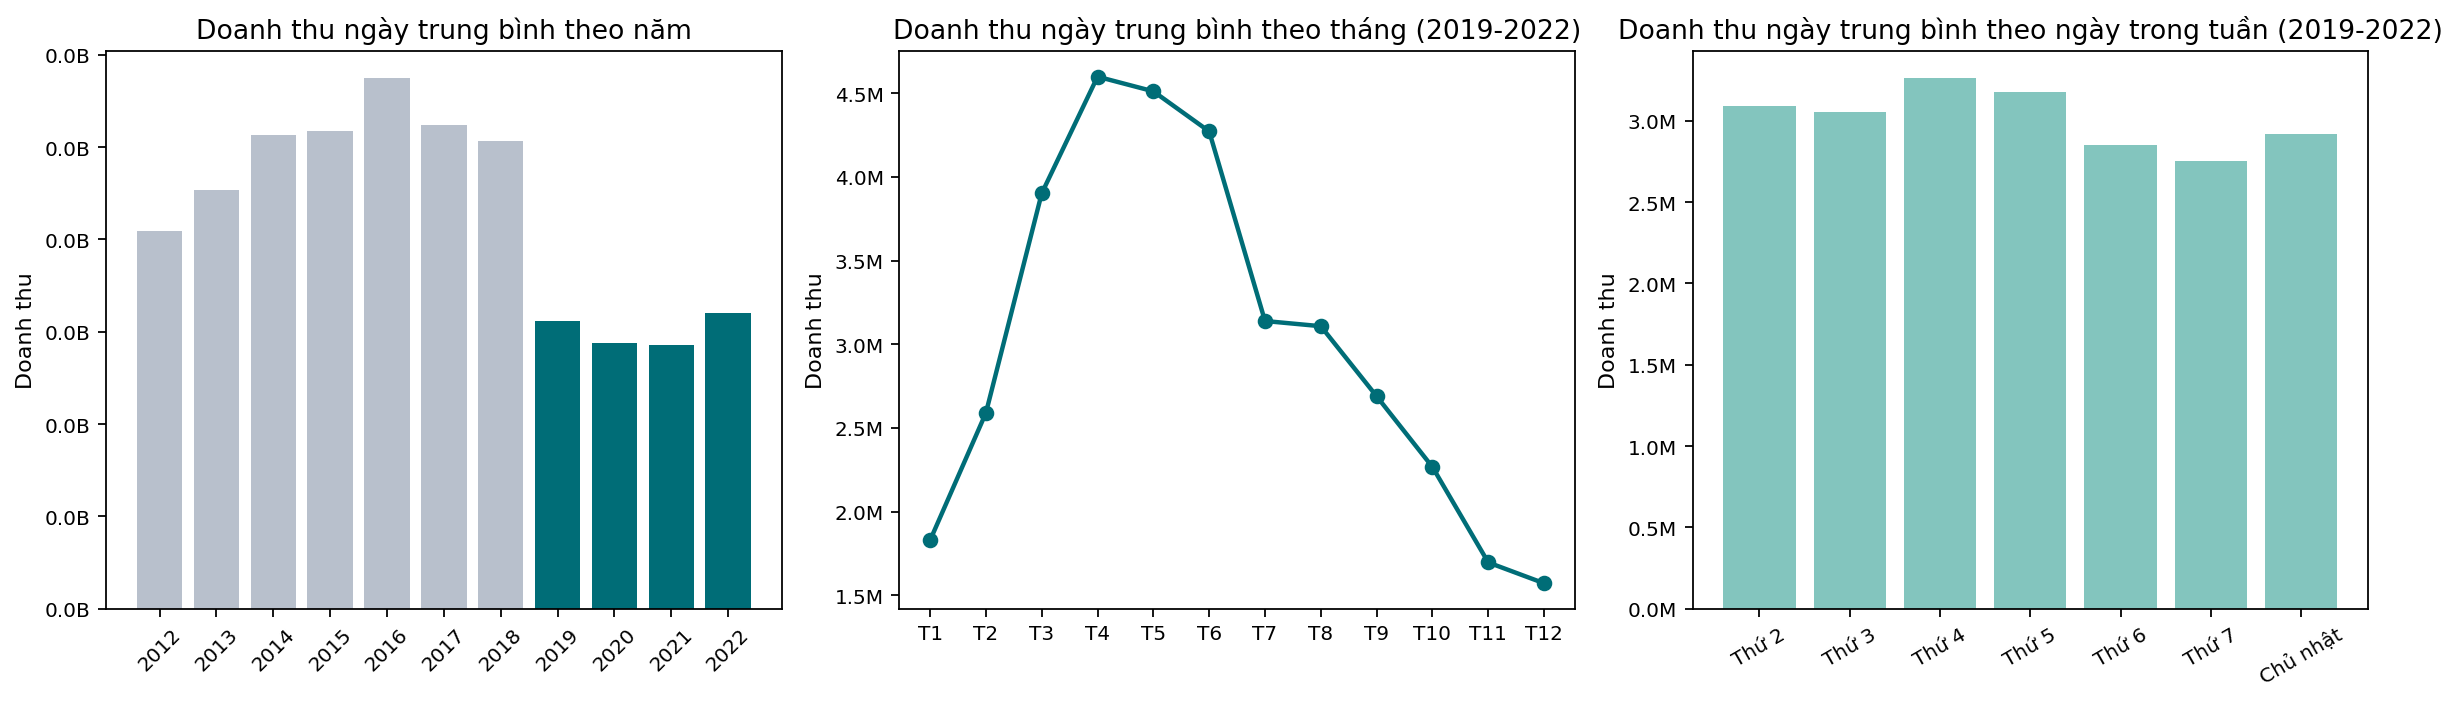
\includegraphics[width=\textwidth]{assets/demand_baseline.png}
  \caption{Nền cầu cơ bản. Trái: doanh thu ngày trung bình theo năm cho thấy bước ngoặt cấu trúc rõ rệt sau 2018. Giữa: mùa vụ theo tháng vẫn rất mạnh trong giai đoạn sau 2019. Phải: hiệu ứng theo ngày trong tuần có tồn tại nhưng yếu hơn mùa vụ theo tháng.}
  \label{fig:demand}
\end{figure*}

\subsection{Số đơn và tỷ lệ chuyển đổi quan trọng hơn lưu lượng truy cập thô}
Doanh thu ngày gắn với số đơn hàng mạnh hơn rất nhiều so với lưu lượng truy cập đầu phễu. Chúng tôi đo được $\mathrm{corr}(\text{Revenue}, \text{Orders})=0.9359$, $\mathrm{corr}(\text{Revenue}, \text{Conversion Proxy})=0.6259$, trong khi $\mathrm{corr}(\text{Revenue}, \text{Sessions})=0.3211$. Điều này gợi ý rằng doanh nghiệp sẽ được lợi nhiều hơn nếu tối ưu tỷ lệ chuyển đổi và chất lượng trưng bày hàng hóa, thay vì chỉ mua thêm lượt truy cập không phân biệt. Ở góc độ bảng theo dõi, nên theo dõi đồng thời orders, conversion và AOV thay vì chỉ tập trung vào sessions.

\subsection{Doanh nghiệp đã tích lũy được nền tảng khách hàng trung thành --- thách thức là tần suất mua, không phải giữ chân}
Doanh nghiệp đã xây dựng được tập khách quen: \SI{75.2}{\percent} khách hàng đặt hơn một đơn, và giai đoạn 2019--2022, \SI{95.8}{\percent} tổng đơn đến từ khách quay lại. Tuy nhiên, heatmap cohort (Hình~\ref{fig:cohort}) tiết lộ một xu hướng đáng lo: tỷ lệ mua lại M+12 của cohort 2013 đạt \SI{8.1}{\percent} nhưng giảm đều xuống còn \SI{0.3}{\percent} ở cohort 2020 --- suy giảm hơn 25 lần trong một thập kỷ. Điều đáng chú ý hơn: với mỗi cohort, tỷ lệ M+1 và M+12 gần bằng nhau (ví dụ cohort 2016: M+1~=~\SI{3.2}{\percent}, M+12~=~\SI{2.6}{\percent}), nghĩa là gần như không có tích lũy lòng trung thành theo thời gian --- khách nào mua lại thì mua sớm trong năm đầu, khách nào không mua trong năm đầu thì không mua nữa. Đây phản ánh đặc tính mua theo sự kiện/mùa vụ của thời trang, không phải churn theo nghĩa thông thường, nhưng xu hướng suy giảm liên tục qua các cohort là tín hiệu cần điều tra: liệu sản phẩm mới có đang kém hấp dẫn khách cũ hơn không? Hàm ý vận hành: tại cuối dữ liệu có \num{1675} khách đang trong vùng 60--90 ngày im lặng --- nhóm có xác suất mua lại cao nhất nếu được tiếp cận đúng lúc qua chiến dịch re-engagement, đặc biệt ở nhóm Streetwear chiếm \SI{79.9}{\percent} doanh thu.

\begin{figure}[htbp]
  \centering
  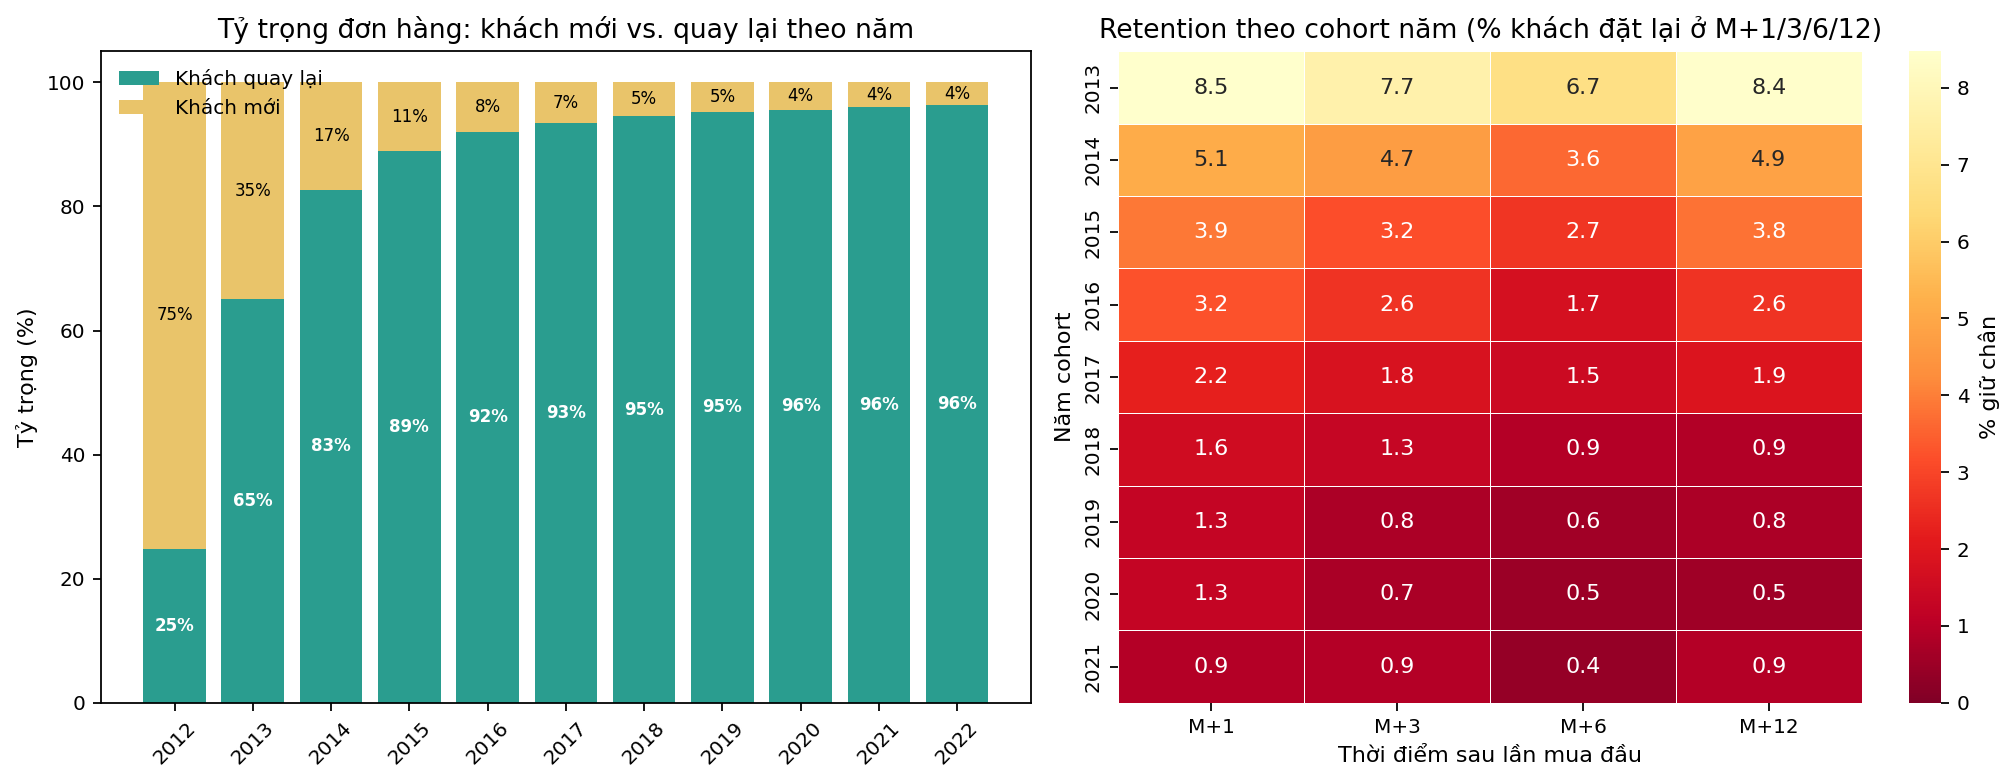
\includegraphics[width=\columnwidth]{assets/cohort_retention.png}
  \caption{Retention khách hàng. Trái: tỷ trọng đơn hàng theo năm. Phải: heatmap retention theo cohort năm --- tỷ lệ khách đặt lại trong M+1, M+3, M+6, M+12.}
  \label{fig:cohort}
\end{figure}

\subsection{Khuyến mãi có tạo doanh thu, nhưng giảm số tiền cố định đang phá biên lợi nhuận}
Khuyến mãi là một phần lớn của động cơ thương mại, nhưng hồ sơ lợi nhuận khác nhau rất mạnh theo từng cơ chế (Hình~\ref{fig:promo}). Khuyến mãi dạng percentage vẫn giữ biên lợi nhuận gộp dương khoảng \SI{5.98}{\percent}, trong khi khuyến mãi dạng fixed tạo khoảng \num{376.5}M VND doanh thu nhưng phá huỷ khoảng \num{230.5}M VND lợi nhuận gộp, tương đương biên lợi nhuận gộp \SI{-61.2}{\percent}. Bài học rút ra không phải là xoá toàn bộ khuyến mãi, mà là phải thiết kế lại cơ cấu khuyến mãi. Hành động khẩn cấp nhất là rà soát hoặc đặt ngưỡng cho nhóm khuyến mãi giảm tiền cố định trước khi cắt rộng toàn bộ chương trình giảm giá.

\begin{figure}[htbp]
  \centering
  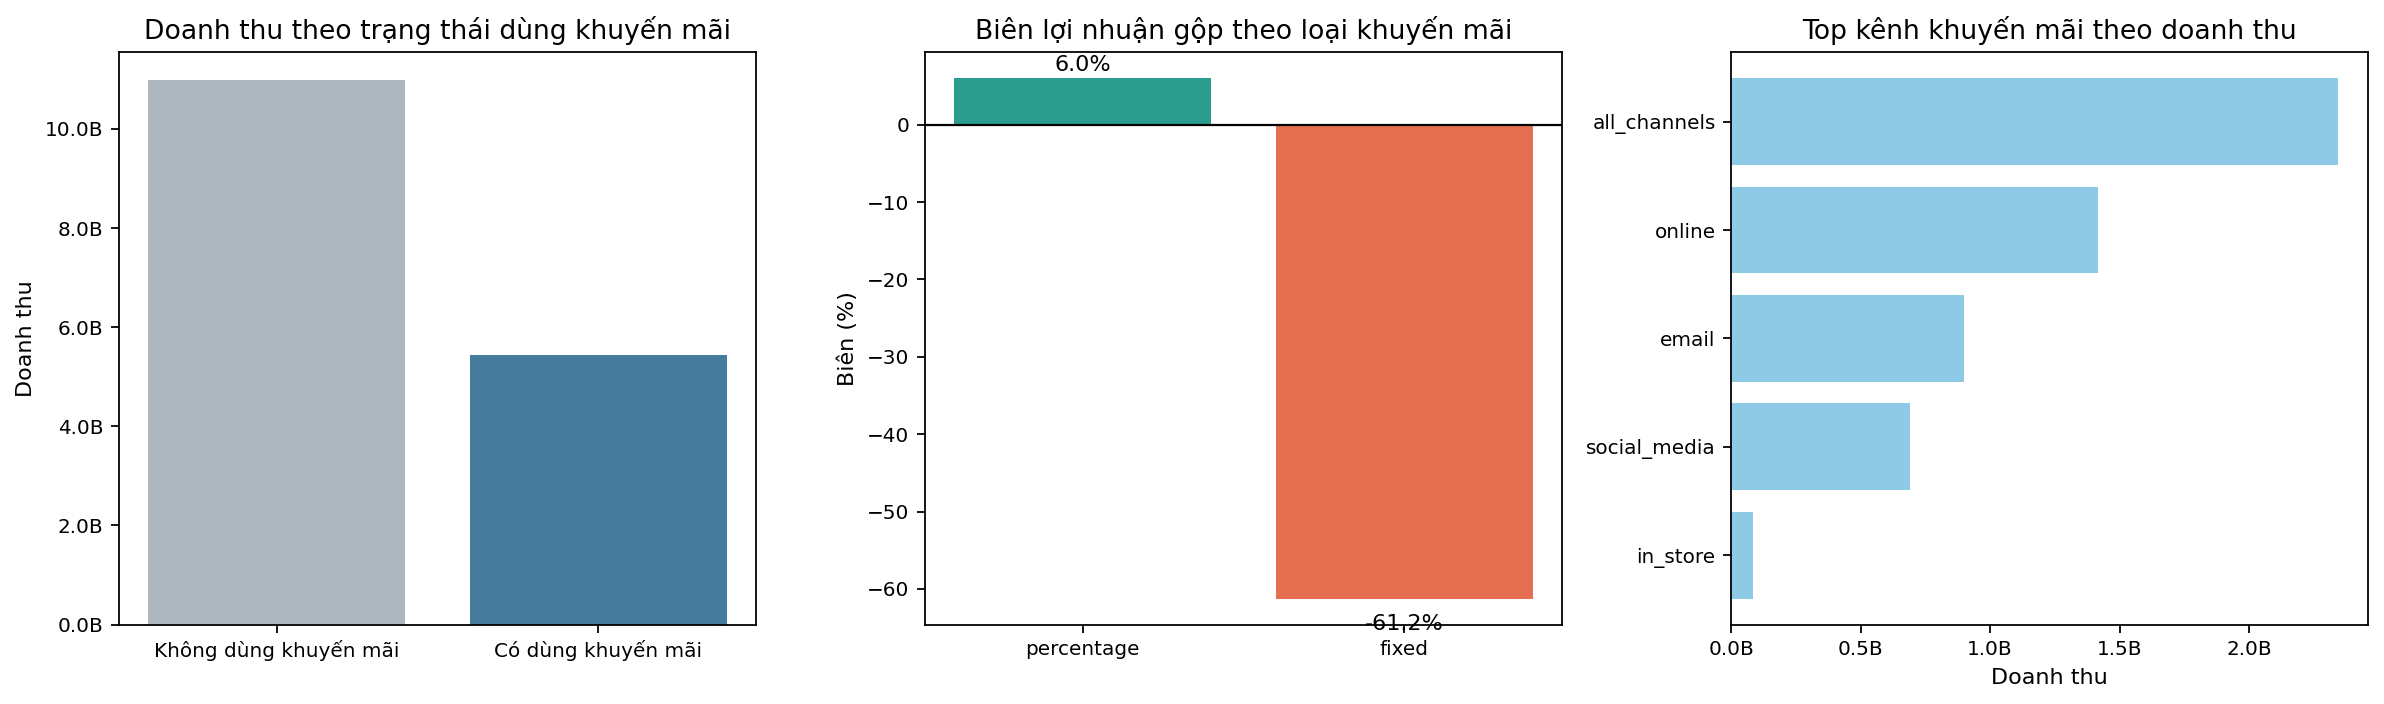
\includegraphics[width=\columnwidth]{assets/promo_economics.png}
  \caption{Kinh tế học khuyến mãi. Khuyến mãi tạo ra doanh thu đáng kể, nhưng không phải loại nào cũng tốt cho biên lợi nhuận.}
  \label{fig:promo}
\end{figure}

\subsection{COD và wrong-size là hai điểm rò rỉ doanh thu lớn nhất}
Ma sát thương mại xuất hiện sau khi nhu cầu đã được tạo ra (Hình~\ref{fig:friction}). COD có tỷ lệ huỷ đơn cao nhất ở mức \SI{16.0}{\percent}, so với \SI{7.98}{\percent} của thẻ tín dụng. Nếu kéo COD về mức huỷ đơn tương đương credit card, doanh nghiệp có thể bảo toàn khoảng \num{197.5}M VND doanh thu. Ở phía trả hàng, \texttt{wrong\_size} chiếm khoảng \SI{35}{\percent} số dòng trả hàng, biến sizing và truyền đạt độ vừa vặn thành ưu tiên vận hành hàng đầu.

Mức độ tập trung theo danh mục khiến vấn đề này còn quan trọng hơn: Streetwear đóng góp \SI{79.9}{\percent} doanh thu và \SI{79.6}{\percent} giá trị hoàn tiền. Chỉ cần giảm \SI{10}{\percent} hoàn tiền do sai size ở Streetwear đã có thể tiết kiệm khoảng \num{14.0}M VND. Biên GP thực của Streetwear (sau COGS, giảm giá và hoàn tiền) chỉ đạt \SI{5.5}{\percent} --- thấp nhất trong tất cả các danh mục --- trong khi GenZ đạt \SI{11.2}{\percent} dù chỉ chiếm \SI{2.1}{\percent} doanh thu. Mỗi điểm phần trăm cải thiện tỷ lệ hoàn tiền Streetwear sẽ tác động trực tiếp vào biên lợi nhuận.

\begin{figure}[htbp]
  \centering
  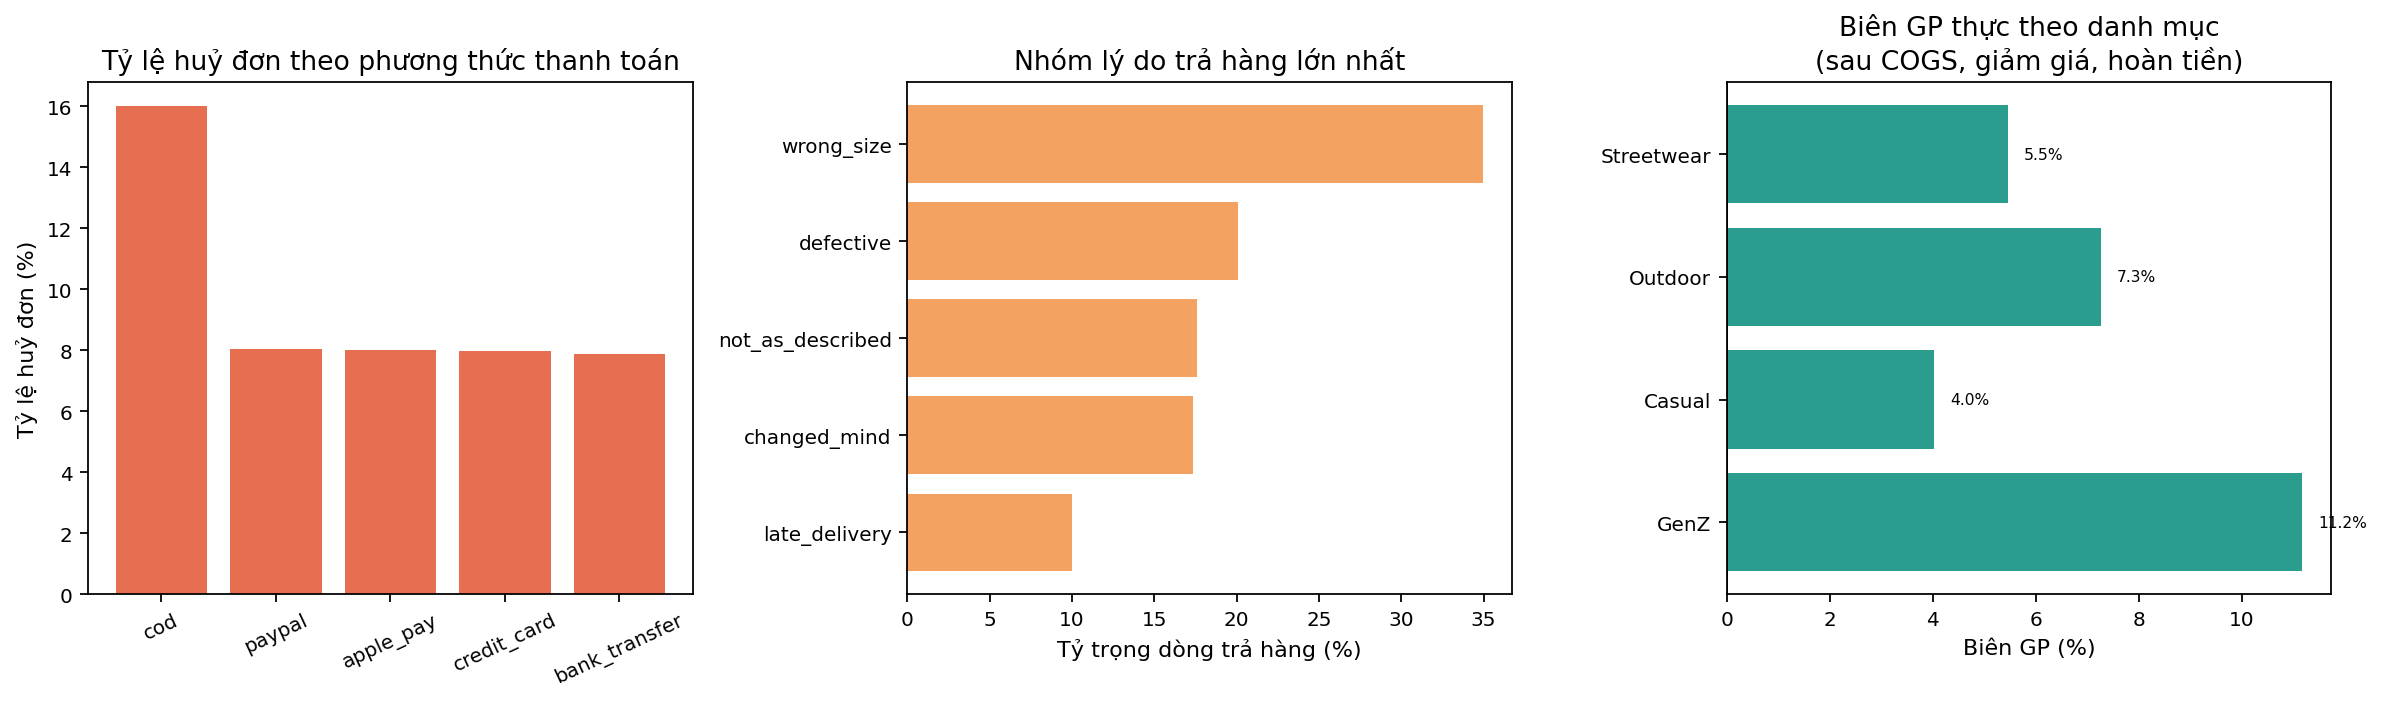
\includegraphics[width=\columnwidth]{assets/returns_cancellations.png}
  \caption{Ma sát thương mại và biên GP theo danh mục. Trái: COD có tỷ lệ huỷ đơn cao nhất. Giữa: \texttt{wrong\_size} chiếm ưu thế về lý do trả hàng. Phải: biên GP thực từng danh mục sau COGS, giảm giá và hoàn tiền --- Streetwear (\SI{79.9}{\percent} doanh thu) có biên thấp nhất ở \SI{5.5}{\percent}.}
  \label{fig:friction}
\end{figure}

\subsection{Bất cân xứng tồn kho là bài toán phân bổ, không chỉ là thiếu hàng}
Streetwear vừa là động cơ doanh thu lớn nhất, vừa là cụm tập trung hoàn tiền lớn nhất (Hình~\ref{fig:portfolio}). Đồng thời, danh mục này còn cho thấy áp lực tồn kho rất cao: \texttt{stockout\_flag} trung bình ở mức \SI{67.3}{\percent}, \texttt{overstock\_flag} ở mức \SI{74.9}{\percent}, và \texttt{days\_of\_supply} khoảng 887 ngày. Outdoor còn cực đoan hơn về số ngày đủ hàng, khoảng 1068.8 ngày. Việc stockout và overstock cùng xuất hiện cho thấy bài toán không nằm ở tổng tồn kho nói chung, mà nằm ở phân bổ sai giữa các danh mục, cơ cấu SKU và các mùa bán.

\begin{figure}[htbp]
  \centering
  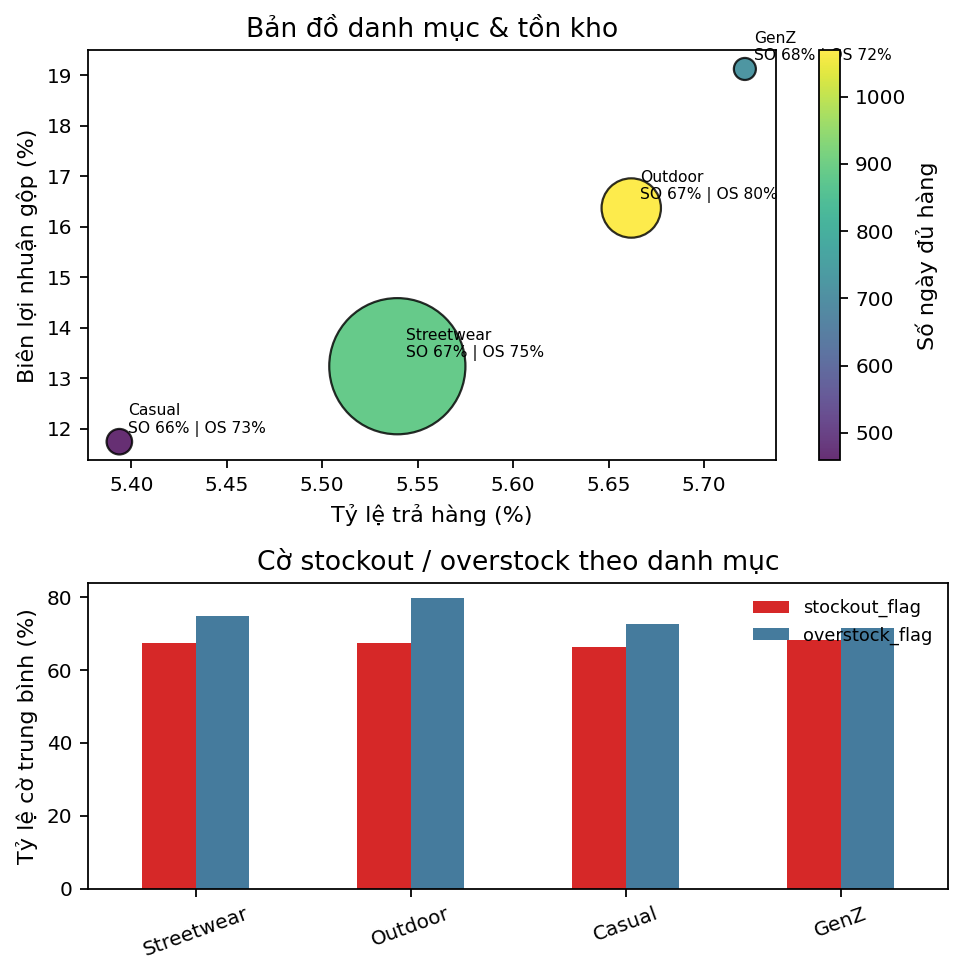
\includegraphics[width=\columnwidth]{assets/category_portfolio.png}
  \caption{Bản đồ danh mục và tồn kho. Trên: bong bóng phản ánh tỷ trọng doanh thu; màu phản ánh số ngày đủ hàng; nhãn kèm tỷ lệ stockout/overstock theo danh mục. Dưới: cờ stockout và overstock trung bình theo danh mục. Streetwear chi phối cả giá trị tạo ra lẫn rủi ro vận hành.}
  \label{fig:portfolio}
\end{figure}

\subsection{Biên lợi nhuận thực và chất lượng kênh giúp ưu tiên ngân sách đúng chỗ}
Hình~\ref{fig:margin_channel} gộp hai section cuối của notebook analytics: section~8 về biên GP thực và section~9 về chất lượng kênh. Ở phía danh mục, Streetwear lớn nhất về doanh thu nhưng lại có biên GP thực thấp nhất sau khi trừ COGS, giảm giá và hoàn tiền; vì vậy danh mục này không thể được quản chỉ bằng top-line revenue. Ở phía kênh, chênh lệch giữa AOV và tỷ lệ huỷ cho thấy không phải kênh nào tạo đơn lớn cũng tạo giá trị tốt: ngân sách nên được giữ ở nhóm kênh có AOV cao và huỷ thấp, thay vì dàn đều theo volume.

\begin{figure}[htbp]
  \centering
  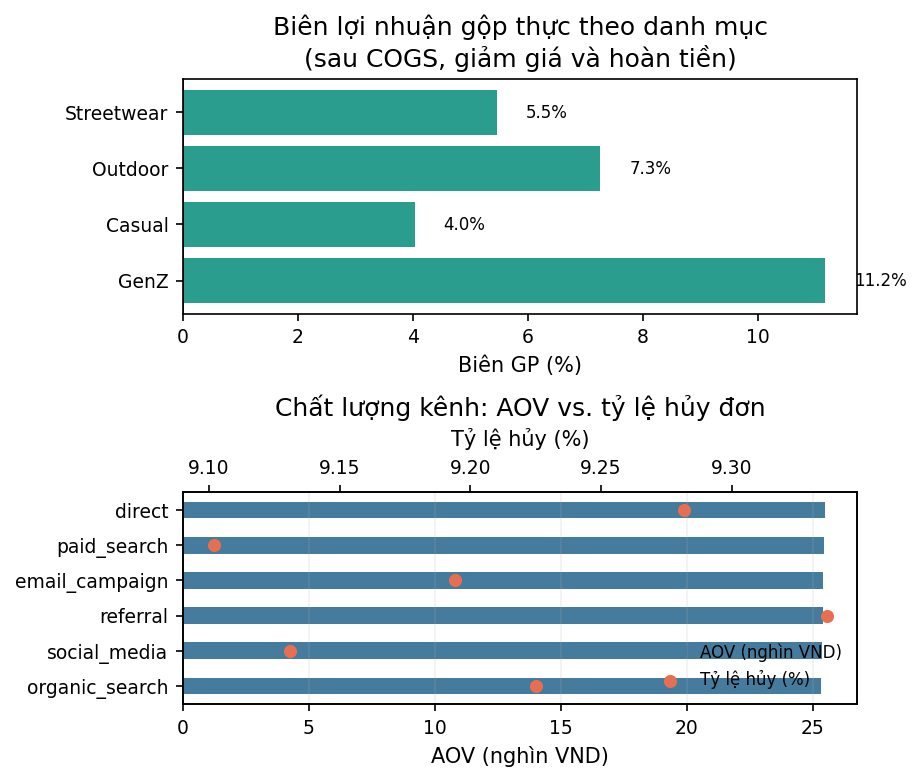
\includegraphics[width=\columnwidth]{assets/margin_channel.png}
  \caption{Biên lợi nhuận thực và chất lượng kênh. Trên: biên GP thực theo danh mục sau COGS, giảm giá và hoàn tiền. Dưới: AOV và tỷ lệ huỷ theo kênh.}
  \label{fig:margin_channel}
\end{figure}

\subsection{Các hành động ưu tiên}
\noindent Bảng~\ref{tab:actions} chốt lại thứ tự ưu tiên từ các section analytics phía trên. Hai việc có tác động tiền mặt ngắn hạn lớn nhất vẫn là tái thiết kế khuyến mãi fixed-amount và kéo tỷ lệ huỷ COD về gần mức thẻ. Các việc sizing và tái phân bổ tồn kho Streetwear nhỏ hơn về giá trị ngắn hạn, nhưng là điều kiện để cải thiện biên thực bền hơn.

\begin{table}[t]
  \centering
  \caption{Danh sách hành động ưu tiên, sắp theo giá trị kinh tế ước tính.}
  \label{tab:actions}
  \scriptsize
  \begin{tabular}{p{0.33\columnwidth} p{0.12\columnwidth} p{0.18\columnwidth} p{0.14\columnwidth}}
    \toprule
    Hành động & Giá trị & KPI & Owner \\
    \midrule
    Thiết kế lại hoặc dừng khuyến mãi fixed-amount & 230.5M & GP theo promo & Fin. / Mktg \\
    Kéo tỷ lệ huỷ COD về gần mức thẻ & 197.5M & Tỷ lệ huỷ COD & Operations \\
    Giảm 10\% hoàn tiền wrong-size của Streetwear & 14.0M & Giá trị hoàn tiền & Merch. \\
    Tái phân bổ tồn kho Streetwear & Rủi ro vận hành & stockout / overstock & Ops/Inv. \\
    \bottomrule
  \end{tabular}
\end{table}

\FloatBarrier
\section{Phần 3: Pipeline dự báo}
Với bài toán dự báo, chúng tôi dự báo \texttt{Revenue} và \texttt{COGS} cho giai đoạn 2023-01-01 đến 2024-07-01 chỉ bằng dữ liệu được cung cấp. Kiến trúc mô hình kết hợp LightGBM~\citep{ke2017lightgbm} với Prophet~\citep{taylor2018forecasting}. Biến đầu vào bao gồm tín hiệu lịch, mã hóa chu kỳ, hồ sơ mùa vụ và cờ sự kiện như Tết hoặc các đợt sale lớn.

\subsection{Kiểm soát leakage và thiết kế validation}
Chúng tôi bám sát các ràng buộc của đề bài:
\begin{itemize}
  \item \textbf{Không leakage từ test:} không dùng Revenue hoặc COGS tương lai làm input.
  \item \textbf{Không dùng dữ liệu ngoài:} toàn bộ sự kiện và biến đầu vào đều được tạo từ bộ dữ liệu được cấp.
  \item \textbf{Tái lập được:} random seed được cố định và notebook chứa đầy đủ pipeline.
\end{itemize}

Quyết định kỹ thuật quan trọng nhất là giao thức validation. Chúng tôi dùng \texttt{TimeSeriesSplit(n\_splits=2, test\_size=548)} để horizon validation khớp với horizon triển khai thực tế. Hồ sơ mùa vụ được dựng lại trong từng fold, và các dòng train dùng leave-one-year-out seasonal encoding để tránh target-encoding leakage. Thiết kế này bảo thủ hơn setup CV 365 ngày trước đây, nhưng phản ánh thực tế leaderboard tốt hơn.

\subsection{Kết quả và khả năng giải thích}
\begin{table}[t]
  \centering
  \caption{Kết quả cross-validation dưới backtest 548 ngày trung thực hơn với bối cảnh triển khai.}
  \label{tab:forecast}
  \small
  \begin{tabular}{lccc}
    \toprule
    Mục tiêu & R$^2$ & MAE & MAPE \\
    \midrule
    Revenue & 0.5685 & \num{791702} & 33.5\% \\
    COGS & 0.6023 & \num{686117} & 38.1\% \\
    \bottomrule
  \end{tabular}
\end{table}

Mô hình tổ hợp cuối cùng dùng trọng số đã re-tune dưới setup CV trung thực này: \texttt{0.75 LightGBM + 0.25 Prophet} cho Revenue, và \texttt{0.90 LightGBM + 0.10 Prophet} cho COGS. Khả năng giải thích của mô hình được xử lý bằng SHAP~\citep{lundberg2017unified}, qua đó xác nhận các biến mùa vụ và sự kiện thật sự là động lực kinh doanh thay vì chỉ là nhiễu kỹ thuật. Điều này quan trọng cả cho báo cáo lẫn cho việc rà lỗi rủi ro ngoại suy hoặc leakage.

\section{Kết luận và giới hạn}
Bài nộp kết hợp phân tích kinh doanh mang tính hành động với pipeline dự báo được thiết kế cẩn thận: thiết kế lại khuyến mãi giảm tiền cố định, giảm thất thoát COD và ưu tiên sizing cùng phân bổ tồn kho Streetwear là ba đòn bẩy có thể triển khai ngay. Giới hạn chính: không có tín hiệu ngoại sinh cho 2023--2024, một số phát hiện analytics vẫn mang tính tương quan hơn nhân quả, và tồn kho chỉ là snapshot cuối tháng.

\bibliographystyle{plainnat}
\bibliography{round1_refs}

\end{document}
